\chapter{Architettura ed Implementazione}
L'applicazione è stata progettata seguendo un approccio modulare, per consentire una migliore leggibilità del codice e una più facile manutenibilità dello stesso. L'applicazione è composta da vari moduli:
\begin{description}
\item[Socket Manager:] gestione delle connessioni TCP.
\item[Tortella Protocol:] definizione del protocollo utilizzato.
\item[Http Manager:] creazione dei pacchetti http e relativi parser.
\item[Packet Manager:] intermediario tra il livello http e quello dei socket.
\item[Route Manager:] gestione delle regole di routing per i pacchetti di flooding.
\item[Servent:] strutture e funzionalità relative ai peer.
\item[Data Manager:] gestione dei dati della chat e degli utenti.
\item[Init:] modulo che consente il boot iniziale dell'applicazione.
\item[Controller:] gestione della comunicazione tra la GUI e gli strati sottostanti dell'applicazione.
\item[GUI:] generazione e gestione dell'interfaccia grafica.
\end{description}
Moduli di supporto:
\begin{description}	
\item[Utils:] generazione degli id, dump dei dati. 
\item[Common:] definizione dei tipi di dati utilizzati.
\item[Logger:] gestione del log dell'applicativo.
\item[Conf Manager:] gestione del file di configurazione.
\end{description}
\begin{figure}[H]
\begin{center}
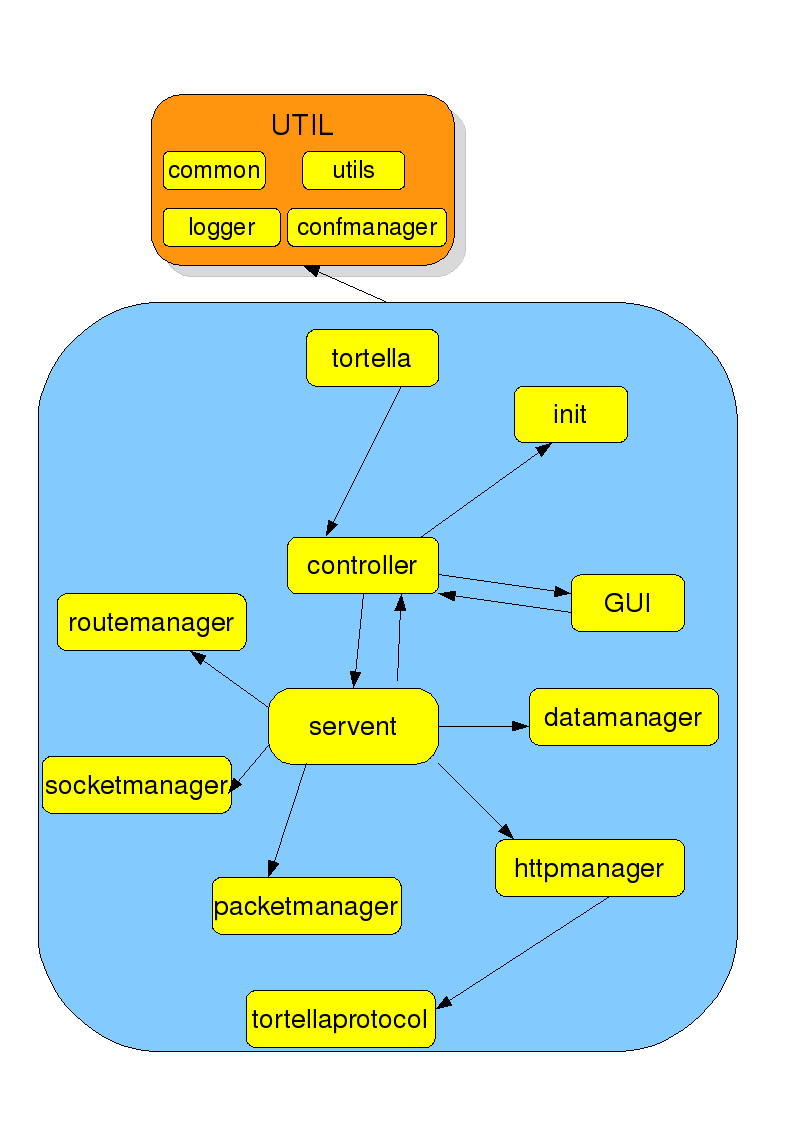
\includegraphics[scale=0.5]{etc/architectural_overview.png}
\caption{Schema Architetturale}
\label{schemaarchitetturale}
\end{center}
\end{figure}
Nella figura \ref{schemaarchitetturale} si possono notare le interdipendenze tra moduli, in particolare l'importanza del modulo servent, che rappresenta il cuore dell'applicazione. Di fondamentale importanza è anche il controller, che gestisce la comunicazione tra la GUI e il resto dell'applicazione, nonchè il bootstrap con le relative connessioni iniziali ai peer.
\section{Socket Manager}
Lo strato software che gestisce l'instaurazione di una connessione di tipo persistente, e di tutto il relativo processo di comunicazione tra due o piu nodi viene gestito dal file socketmanager.c. Poichè un servente deve comportarsi sia da client che da server. A tal proposito verranno analizzate i due processi di creazione dei socket.
\paragraph{create\_tcp\_socket()}
La funzione ha il compito di creare un socket di connessione remota, ovvero di instaurare una connessione remota ad un server TCP. Come è possibile capire il tipo di comunicazione è orientata alla connessione, permettendo il trasferimento di un flusso continuo di dati.
Dopo la fase di inizializzazione del socket e l'apertura della connessione verso il server, viene eseguita la chiamata di sistema setsockopt() con il flag SO\_KEEPALIVE , al fine di caratterizzare la connessione precedentemente instaurata, ovvero creando un tipo di connessione persistente\footnote{Per connessione persistente si intende la presenza di un timer che viene reinizializzato ogni volta che avviene uno scambio di informazioni tra peer. Allo scadere del timer, il socket viene chiuso}.
\begin{lstlisting}
int create_tcp_socket(const char* dst_ip, int dst_port)
\end{lstlisting}
\paragraph{create\_listen\_tcp\_socket} 
Il compito di inizializzare il lato server del peer, creando un un socket d'ascolto, è affidato alla funzione sopra riportata. Dopo l'istanziazione del socket, vengono effettuate le chiamate bind() e listen(), le quali hanno il compito rispettivamente di inizializzare l'indirizzo IP locale e il relativo processo e di porre il socket dallo stato di CLOSED a quello di LISTEN. Come nel caso precedente viene utilizzata la syscall setosockopt(), la quale non si occupa solo di mantenere la connessione in uno stato permanente, ma anche di poter riutilizzare l'indirizzo locale. Usando il flag \texttt{SO\_REUSEADDR} fra la chiamata a socket() e quella a bind() si consente a quest'ultima di avere comunque successo anche se la connessione è attiva o si trova nello stato di TIME\_WAIT.  
Le operazioni riguardanti la ricezione del flusso di pacchetti e relativo invio  sono gestite rispettivamente dalle funzioni: recv\_packet(), send\_packet(), le quali attraverso le chiamate di sistema standard della programmazione di rete si occupano di svolgere le funzioni di scrittura e lettura sui sockets d'interesse. Particolare attenzione deve essere rivolta alla funzione di lettura dei dati, in quanto è stato previsto un meccanismo di frammentazione dei pacchetti in blocchi, di dimensione massima (4096 byte) pari a quella impostata nel parametro buffer\_len, presente nel file di configurazione iniziale (tortella.conf).
\begin{lstlisting}
int create_listen_tcp_socket(const char* src_ip, int src_port)
\end{lstlisting}
Il modulo, oltre alle funzioni di creazione del socket, fornisce le funzioni relative all'invio e alla ricezione dei pacchetti.
\paragraph{send\_packet()}
Tale funzione consente la comunicazione tra i peer, in particolare consente di inviare dati tramite un socket. Per effettuare questa operazione viene utilizzata la chiamata di sistema \texttt{write()}.
\begin{lstlisting}
int send_packet(int sock_descriptor, char* buffer, int len)
\end{lstlisting}
\paragraph{recv\_packet()}
Quest'ultima funzione consente la ricezione dei dati da un peer. E' stata progettata rendendo possibile la ricezione di dati di dimensione illimitata (teoricamente), questo per rendere possibile il trasferimento di grossi file\footnote{funzionalità non implementata}. Il buffer passato come argomento deve essere non allocato per consentire alla funzione di allocare memoria dinamicamente.
\begin{lstlisting}
int recv_sized_packet(int sock_descriptor,char** buf, int max_len)
\end{lstlisting}
\section{Tortella Protocol}
Questo modulo contiene tutte le definizioni, le funzioni e le macro che implementano il protocollo TorTella. Ci sono tutte le definizioni dei pacchetti e dei descrittori trasportati, che sono i seguenti:
\begin{lstlisting}[frame=single]
#define PING_ID			0x01
#define LIST_ID			0x03
#define LISTHITS_ID		0x04
#define JOIN_ID			0x05
#define LEAVE_ID		0x06
#define MESSAGE_ID		0x07
#define SEARCH_ID		0x09
#define SEARCHHITS_ID	0x10
#define BYE_ID			0x11
#define CLOSE_ID 		0x12

//Status ID
#define ONLINE_ID	0x80
#define BUSY_ID		0x81
#define AWAY_ID		0x82

struct tortella_header {
	u_int8 id;		
	u_int4 desc_id;
	u_int8 sender_id;   
	u_int8 recv_id; 
	time_t timestamp;
	u_int4 desc_len; 
	u_int4 data_len; 
};
typedef struct tortella_header tortella_header;

struct ping_desc {
	u_int4 port;
	u_int1 status;
	//Cambo dati: nickname
};
typedef struct ping_desc ping_desc;

struct list_desc {
	u_int8 chat_id;	
	u_int1 ttl;
	u_int1 hops;
};
typedef struct list_desc list_desc;

struct listhits_desc {
	u_int4 user_num;	
	u_int1 ttl;
	u_int1 hops;
	u_int8 chat_id;
	//Campo dati: elenco utenti della chat
};
typedef struct listhits_desc listhits_desc;

struct join_desc {
	u_int1 status;
	u_int8 user_id;
	u_int8 chat_id; 
	u_int4 port;
	char ip[16];
	u_int1 ttl;
	u_int1 hops;
	//Campo dati: nickname
};
typedef struct join_desc join_desc;

struct leave_desc {
	u_int8 user_id;
	u_int8 chat_id; 
	u_int1 ttl;
	u_int1 hops;
};
typedef struct leave_desc leave_desc;

struct message_desc {
	u_int8 chat_id;		
	//Campo dati: il msg
};
typedef struct message_desc message_desc;

struct search_desc {
	u_int1 ttl;
	u_int1 hops;
	//Campo dati: stringa ricerca
};
typedef struct search_desc search_desc;

struct searchhits_desc {
	u_int4 num_res;
	//Campo dati: risultati ricerca
};
typedef struct searchhits_desc searchhits_desc;

struct bye_desc {
};
typedef struct bye_desc bye_desc;

struct tortella_packet {
	tortella_header *header;
	char *desc;	//desc_len nell'header del pacchetto
	char *data;	//data_len nell'header del pacchetto
};
typedef struct tortella_packet tortella_packet;
\end{lstlisting}
Le varie funzioni sono descritte di seguito:
\paragraph{tortella\_bin\_to\_char()}
Questa funzione ha il compito di eseguire il parser del pacchetto tortella. In particolare prende in input da parametro il pacchetto, memorizzato nella sua struttura dati, e restituisce tutto il suo contenuto in un buffer di caratteri. Inoltre ritorna la lunghezza del buffer generato. Si è cercato di rendere tale operazione di conversione il più efficiente possibile, essendo una funzionalità utilizzata ogni volta che si invia un pacchetto.
\begin{lstlisting}
char *tortella_bin_to_char(tortella_packet *packet, u_int4 *len)
\end{lstlisting}
\paragraph{tortella\_char\_to\_bin()}
Tale funzione svolge le funzionalità di parser inverso rispetto alla funzione \texttt{tortella\_bin\_to\_char()}. La procedura riceve come parametro il buffer, contenente i dati, i quali vengono memorizzati nella struttura dati \texttt{tortella\_packet}. Questa funzione viene chiamata ogni volta che si riceve un pacchetto, per estrarre il suo contenuto e renderlo maggiormente accessibile dalle altre funzioni del programma.
\begin{lstlisting}
tortella_packet *tortella_char_to_bin(char *packet)
\end{lstlisting}
\section{Http Manager}
La gestione dei pacchetti HTTP, il cui protocollo è stato definito nel precedente capitolo, viene affrontato all'interno di questo modulo. Di seguito vengono riportate le strutture dati rappresentanti i pacchetti:
\begin{lstlisting}
struct http_header_request {
	char *request;
	char *user_agent;
	u_int4 range_start;
	u_int4 range_end;
	u_int4 content_len;
	char *connection;
};
typedef struct http_header_request http_header_request;

struct http_header_response {
	char *response;
	char *server;
	char *content_type;
	u_int4 content_len;
};
typedef struct http_header_response http_header_response;

struct http_packet {
	u_int4 type;
	http_header_request *header_request;
	http_header_response *header_response;
	tortella_packet *data;
	char *data_string;
	u_int4 data_len;
};
typedef struct http_packet http_packet;
\end{lstlisting}
Come è possibile notare sono state definite 3 tipi di strutture dati, dove le prime due sono utilizzate per la creazione dell'header a seconda se il messaggio da inviare si di richiesta o di risposta, invece la terza struttura è utilizzata per definire l'intero pacchetto http. Sia nell'header di request che nell'header di response viene memorizzata, la lunghezza dell'intero pacchetto, la tipologia di dei dati contenuti(html,image..), che nel nostro caso saranno solamente di tipo binario e la versione del tipo di protocollo utilizzato (Tortella 0.1). Le uniche differenze presenti sono dovute, al tipo di informazione (richiesta o risposta) contenuta negli headers, e all'identificazione nell'header request del tipo di connessione instaurata (di tipo persistente) tra due peer.
Al fine di rendere più agevole la creazione di un generico pacchetto sono state definite delle macro all'interno dell header file:
\begin{lstlisting}
#define HTTP_REQ_GET		0x40
#define	HTTP_RES_GET		0x41
#define HTTP_REQ_POST		0x42
#define HTTP_RES_POST		0x43
#define HTTP_STATUS_OK		200
#define	HTTP_STATUS_CERROR	400
#define HTTP_STATUS_SERROR	500

#define HTTP_REQ_POST_LINE	"POST * HTTP/1.1"
#define HTTP_AGENT			"User-Agent: "
#define HTTP_REQ_RANGE		"Range: bytes="
#define HTTP_CONNECTION		"Connection: "
#define HTTP_CONTENT_TYPE	"Content-Type: "
#define HTTP_CONTENT_LEN	"Content-Length: "
#define HTTP_SERVER			"Server: "

#define HTTP_OK			"HTTP/1.1 200 OK"
#define HTTP_CERROR		"HTTP/1.1 400 Bad Request"
#define HTTP_SERROR		"HTTP/1.1 500 Internal Server Error"
\end{lstlisting}
Tutte le funzionalità relative al parsing dei dati contenuti nel pacchetto http sono svolte dalle seguenti funzioni:
\paragraph{http\_bin\_to\_char()}
La funzione si occupa di leggere i dati memorizzati in una struttura dati per poi salvare gli stessi in un buffer di caratteri. Nel momento in cui vi è la chiamata a tale funzione vengono passati come parametro sia l'intero pacchetto http che la sua lunghezza. L'algoritmo di parsing dopo aver controllato che il pacchetto ricevuto non sia vuoto provvede all'istanziazione di un buffer, il quale avrà dimensioni differenti  in base al tipo di messaggio contenente il pacchetto (REQ\_POST-REQ\_GET-RES\_POST-RES\_GET). Ogni campo dell'header, all'interno del buffer, viene delimitato con due caratteri separatori \texttt{$\setminus r\setminus n$}, in modo da permettere un'identificazione migliore delle varie informazioni, nel caso in cui si abbia la necessità di riconvertire tutti i dati nelle loro strutture d'appartenenza (\texttt{http\_char\_to\_bin}). Dopo di ciò viene fatto uso di un puntatore temporaneo, il quale dopo essere stato inizializzato con l'indirizzo del primo byte del buffer, viene spostato della sua lunghezza, in modo da poter appendere in seguito tutte le informazioni relative al campo dati del pacchetto http (vedi appendice).
\begin{lstlisting}
char *http_bin_to_char(http_packet *packet, int *len)
\end{lstlisting}
\paragraph{http\_char\_to\_bin()}
La funzione esegue il procedimento inverso della \texttt{http\_bin\_to\_char()}, in quanto prendendo da parametro un puntatore a caratteri, che contiene i campi dati del pacchetto http, effettua la conversione di questa nella relativa struttura d'appartenenza. Come nel caso precedente l'algoritmo suddivide il processo di parsing a seconda del tipo di pacchetto da ricostruire. Durante la conversione la funzione si occupa anche di preparare la struttura dati \texttt{tortella\_packet}, fornita dallo strato inferiore come contenitore del messaggio del pacchetto.
\begin{lstlisting}
http_packet *http_char_to_bin(const char *buffer)
\end{lstlisting}
\section{Packet Manager}
Il modulo in questione consente di creare ed inviare pacchetti TorTella e HTTP. Si può considerare come un insieme di API, volte a migliorare la leggibilità del codice, altrimenti si sarebbero dovute effettuare tutte le operazioni di invio manualmente. In particolare, le operazioni che ognuna di queste API svolge sono:
\begin{enumerate}
\item Preparazione dell'header del pacchetto TorTella; 
\item Preparazione del descrittore del pacchetto in base a ciò che si vuole inviare;
\item Preparazione dei dati (qualora presenti) del pacchetto TorTella;
\item Preparazione del pacchetto HTTP;
\item Conversione del pacchetto in un buffer di dati;
\item Invio del pacchetto;
\end{enumerate}
Di seguito si riportano le definizioni delle funzioni:
\begin{lstlisting}
int send_search_packet(u_int4 fd, u_int8 packet_id, u_int8 sender_id, u_int8 recv_id, u_int1 ttl, u_int1 hops, u_int4 string_len, char *string);

int send_searchhits_packet(u_int4 fd, u_int8 packet_id, u_int8 sender_id, u_int8 recv_id, u_int4 num_res, u_int4 res_len, char *res);

int send_join_packet(u_int4 fd, u_int8 packet_id, u_int8 sender_id, u_int8 recv_id, u_int1 status, u_int8 user_id, u_int8 chat_id, char *nick, u_int4 port, char *ip, u_int1 ttl, u_int1 hops);

int send_leave_packet(u_int4 fd, u_int8 packet_id, u_int8 sender_id, u_int8 recv_id, u_int8 user_id, u_int8 chat_id, u_int1 ttl, u_int1 hops);

int send_ping_packet(u_int4 fd, u_int8 sender_id, u_int8 recv_id, char *nick, u_int4 port, u_int1 status);

int send_list_packet(u_int4 fd, u_int8 sender_id, u_int8 recv_id, u_int1 ttl, u_int1 hops, u_int8 chat_id);

int send_listhits_packet(u_int4 fd, u_int8 sender_id, u_int8 recv_id, u_int4 user_num, u_int4 res_len, char *res, u_int8 chat_id);

int send_bye_packet(u_int4 fd, u_int8 sender_id, u_int8 recv_id);

int send_message_packet(u_int4 fd, u_int8 sender_id, u_int8 recv_id, u_int8 chat_id, u_int4 msg_len, char *msg);

int send_post_response_packet(u_int4 fd, u_int4 status, u_int4 data_len, char *data);

int send_get_request_packet(u_int4 fd, char *filename, u_int4 range_start, u_int4 range_end);

int send_get_response_packet(u_int4 fd, u_int4 status, u_int4 data_len, char *data);
\end{lstlisting}
\section{Route Manager}
Il modulo è stato implementato per la gestione delle regole di backward-routing dei pacchetti di tipo Search-SearchHits. Il peer da cui parte la richiesta deve ricevere un pacchetto SearchHits da ogni peer che ha ricevuto la richiesta; per realizzare tale meccanismo si utilizzano le regole di routing. In particolare, ogni peer che riceve un pacchetto Search deve memorizzare nella tabella di routing un record relativo al percorso che dovrà effettuare il SearchHits di risposta.
Per il funzionamento di questo meccanismo è stata utilizzata una hashtable contenente la struttura dati di seguito elencata:
\begin{lstlisting}
struct route_entry {
	u_int8 sender_id;
	u_int8 recv_id;
	u_int4 counter;
};
typedef struct route_entry route_entry;
\end{lstlisting}
Le regole vengono gestite attraverso le seguenti funzioni:
\begin{lstlisting}
int add_route_entry(u_int8 packet_id, u_int8 sender_id, u_int8 recv_id);

int del_route_entry(u_int8 id);

route_entry *get_route_entry(u_int8 packet_id);

u_int8 get_iddest_route_entry(u_int8 id);
\end{lstlisting}
\section{Servent}
L’architettura di un sistema peer‐to‐peer prevede che ogni entità sia in grado di funzionare sia da client che da server. Ogni peer deve quindi essere realizzato come un servent. La parte server dovrà gestire i messaggi in arrivo dalla rete e quella client dovrà invece provvedere a inviare dati agli altri peer. Questo porta alla necessità di avere un sistema di gestione di tipo concorrente. L'utilizzo di thread, per la gestione concorrente delle richieste, 
ha permesso una maggiore agevolazione nella implementazione della comunicazione client-server.
\paragraph{servent\_data}
Per la comunicazione tra i thread relativi ad un peer è stata predisposta una struttura dati per la condivisione delle informazioni, ovvero la \texttt{servent\_data}:
\begin{lstlisting}
struct servent_data {
	u_int8 id;
	GQueue *queue;	
	GQueue *res_queue;
	char *ip;
	u_int4 port;
	u_int1 status;
	char *nick;
	time_t timestamp;
	
	GList *chat_list;

	pthread_rwlock_t rwlock_data;
	
	char *msg;
	u_int4 msg_len;
	
	GList *chat_res;
	u_int1 ttl;
	u_int1 hops;
	u_int8 packet_id;
	
	u_int1 is_online;
	u_int4 post_type;
	
	//FLOODING
	u_int8 user_id_req;
	u_int8 chat_id_req;
	u_int4 port_req;
	char *nick_req;
	char *ip_req;
	u_int1 status_req;
	char *title;
	u_int4 title_len;
};
typedef struct servent_data servent_data;
\end{lstlisting}
I campi della struttura presentata sono divisi in gruppi, in base al loro tipo di utilizzo:
\begin{itemize}
\item i campi che rappresentano le informazioni del peer, come: ip, porta, nickname, id;
\item i campi utilizzati per la comunicazione con il peer, come il tipo di pacchetto da inviare al peer associato alla struttura dati. Ad esempio, nel caso in cui il server thread dovesse riceve un pacchetto Search da uno specifico peer, tale campo dovrà assumere il valore \texttt{SEARCHHITS\_ID} per segnalare al client thread di inviare il pacchetto SearchHits di risposta;
\item i campi utilizzati per il flooding, ovvero servono alla ritrasmissione dei pacchetti ricevuti (Search, SearchHits, Join, Leave).
\end{itemize}
Per l'accesso alla \texttt{servent\_data} di un peer vengono utilizzati dei meccanismi di lock, i quali consentono di evitare inconsistenza dei dati.\\

All'avvio dell'applicazione un'istanza del controller si occupa di chiamare la funzione \texttt{servent\_start()}, la quale ha il compito di inizializzare tutti i parametri del servente locale, di istanziare il lato server dello stesso, mettendolo in attesa di connessioni da altri peer, ed infine di avviare il suo lato client. A tale proposito all'interno della funzione vi sono tre chiamate di funzione,le quali hanno rispettivamente il compito di svolgere le attività elencate precedentemente. Di seguito vengono mostrati le dichiarazioni, presenti nell'header file, delle tre procedure con relativa spiegazione.
\paragraph{servent\_init()}
La funzione, come affermato in precedenza, si occupa di inizializzare i parametri del servente locale, identificando  il suo indirizzo ip, numero di porta e status iniziale, i quali vengono reperiti dal file di configurazione tortella.conf. Inoltre viene inzializzato il mutex relativo alla sua struttura dati
\begin{lstlisting}
int servent_init(char *ip, u_int4 port, u_int1 status)
\end{lstlisting}
\paragraph{servent\_start\_server()}
La funzione ha il compito di avviare il lato server del peer locale. Inizialmente viene creato il server, con la relativa coppia ip-porta, ricevuta da parametro; in seguito viene lanciato un thread, attivando l'esecuzione della funzione \texttt{servent\_listen()}, nella quale è presente un ciclo infinito, in cui viene creato un nuovo thread per ogni richiesta di connessione da nuovi peer.
\begin{lstlisting}
int servent_start_server(char *local_ip, u_int4 local_port)
\end{lstlisting}
\paragraph{servent\_init	\_connection()}
La funzione ha il compito di inizializzare il lato client del servente locale, e di avviare una connessione per ogni peer vicino presente nella lista \texttt{init\_servent}, la quale viene riempita con i dati relativi ai peer vicini inizialmente conosciuti. Il numero di peer considerati come “vicini” per ognuno dei nodi componenti la rete è stato scelto a priori, e  i relativi indirizzi ip e numero di porta sono salvati in un file di configurazione (init\_data.txt). 
\begin{lstlisting}  
int servent_init_connection(GList *init_servent)
\end{lstlisting}
\paragraph{servent\_connect()}
